\chapter{含自旋的两粒子散射 (Two-Particle Scattering with Spin)}\label{ch:spin2p}

在前几章我们讨论了无自旋粒子的散射理论：单粒子在外势中的散射 (第\ref{ch:Smat1P}章风格)，以及两个无自旋粒子之间的散射 (第\ref{ch:scat2p}章风格)。然而，自然界中的大部分粒子 (electron, proton, neutron, $\pi^\pm$ 之外的诸多 hadron, photon $\cdots$) 都具有非平庸的自旋 (spin)。一旦把自旋自由度加进来，散射理论的形式架构需要做相应的扩充：Hilbert 空间增加自旋分量，相互作用 Hamiltonian 可能依赖于自旋 (典型的例子是 spin--orbit coupling 与 nucleon--nucleon 中的 spin--spin coupling)，对不同初末自旋分量散射振幅一般不再相同——它构成一个 \emph{矩阵} $f_{m_s' m_s}(\theta,\phi)$。本章把第\ref{ch:scat2p}章的两粒子散射框架平行地推广到带自旋的情形，并系统地引入极化、求和/平均与密度矩阵语言。本章最后给出旋转不变性的初步评注，更系统的讨论留到第\ref{ch:invariance}章。

本章主要参考 Taylor《Scattering Theory》中关于 spin 的章节。

%==========================================================================
\section{含自旋时的物理图像与一般考虑}\label{sec:spin-overview}

与无自旋情形相比，带自旋的两粒子散射有以下若干新特征：
\begin{itemize}
  \item Hilbert 空间会更复杂：除轨道空间 (positions/momenta) 外还要张量上自旋空间。
  \item Hamiltonian 可能与自旋有关。例如 spin--orbit coupling $\bm S\cdot\bm L$，spin--spin coupling $\bm S_1\cdot\bm S_2$，tensor coupling $(\bm S_1\cdot\hat{\bm x})(\bm S_2\cdot\hat{\bm x})$ 等。
  \item 不同自旋分量的初末态一般会有不同的散射振幅。换言之，散射振幅不再是一个数 $f(\theta,\phi)$，而是作用在自旋空间上的一个有限维矩阵 $F(\bm p'\!\leftarrow\!\bm p)$。
  \item 实际实验中初态自旋常常是非极化的 (unpolarized)，探测器一般也不分辨末态自旋。这要求我们对自旋自由度做适当的求和/平均，这是 polarization-summed / averaged differential cross section 的来源。
\end{itemize}

下面我们逐步展开。

%==========================================================================
\section{带自旋的单粒子 Hilbert 空间}\label{sec:1p-spin-hilbert}

回顾：自旋为 $s$ 的单粒子的 Hilbert 空间是轨道部分与自旋部分的张量积
\begin{equation}
  \Hilb \;=\; \Hilb_{\rm space} \otimes \Hilb_{\rm spin}\,, \qquad
  \Hilb_{\rm space}=L^2(\R^3),\;\; \dim\Hilb_{\rm spin}=2s+1.
  \label{eq:1p-hilbert}
\end{equation}
自旋空间中常用的基矢是 $\Op S_3$ 的本征态：
\begin{equation}
  \Op S_3\, \ket{m} = m\,\ket{m},\qquad m=-s,\,-s+1,\,\cdots,\,s,
  \label{eq:S3-basis}
\end{equation}
基矢一共 $2s+1$ 个。一般的自旋态 $\ket{\chi}\in\Hilb_{\rm spin}$ 可以展成
\begin{equation}
  \ket{\chi}=\sum_{m=-s}^{s}\chi_m\,\ket{m},
  \qquad
  \chi=\begin{pmatrix}\chi_s\\ \chi_{s-1}\\ \vdots\\ \chi_{-s}\end{pmatrix}\in\C^{2s+1}.
  \label{eq:spinor-column}
\end{equation}
即一个 $2s+1$ 维复列矢量 (spinor)。例如自旋 $1/2$ 时
\begin{equation}
  \chi=\begin{pmatrix}\chi_+\\ \chi_-\end{pmatrix},\qquad
  \chi_+=\inn{+}{\chi},\quad \chi_-=\inn{-}{\chi}.
\end{equation}
自旋算符是有限维矩阵，对自旋 $1/2$ 而言 $\bm S=\bm\sigma/2$ ($\hbar=1$)，其中 $\bm\sigma=(\sigma_1,\sigma_2,\sigma_3)$ 为 Pauli matrices。

总 Hilbert 空间 \eqref{eq:1p-hilbert} 的基矢可以选成轨道基与自旋基的张量积：
\begin{equation}
  \ket{\bm p}\otimes\ket{m},\qquad \bm p\in\R^3,\;\; m\in\{-s,\cdots,s\}.
  \label{eq:basis-1p-spin}
\end{equation}
一个一般的态 $\ket\psi$ 可以写成 $2s+1$ 个分量波函数，每个分量是一个普通的空间波函数：
\begin{equation}
  \psi_m(\bm x)=(\bra{\bm x}\otimes\bra{m})\ket\psi.
\end{equation}

%==========================================================================
\section{带自旋的两粒子 Hilbert 空间}\label{sec:2p-spin-hilbert}

两个粒子的总 Hilbert 空间是各自单粒子空间的张量积：
\begin{equation}
  \Hilb \;=\; \Hilb_1\otimes\Hilb_2 \;=\; \bigl(\Hilb_{\rm space}\otimes\Hilb_{\rm spin}\bigr)_1\otimes\bigl(\Hilb_{\rm space}\otimes\Hilb_{\rm spin}\bigr)_2.
  \label{eq:2p-hilbert}
\end{equation}
若用直积基矢 $\ket{\bm x_1,m_1}\otimes\ket{\bm x_2,m_2}$，则一个 (纯态) 波函数有 $(2s_1+1)(2s_2+1)$ 个分量：
\begin{equation}
  \psi_{m_1 m_2}(\bm x_1,\bm x_2) \;=\; \matel{\bm x_1\, m_1;\, \bm x_2\, m_2}{}{\psi}.
  \label{eq:wavefunc-2p-spin}
\end{equation}

\paragraph{质心分解。}与无自旋的情形相同，我们做坐标变换分离质心运动与相对运动 (orbital part)，自旋部分则不动 (它与位置算符独立)：
\begin{equation}
  \begin{aligned}
    \Hilb \;&=\; \bigl(\Hilb_{\rm space,cm}\otimes\Hilb_{\rm space,rel}\bigr)\otimes \bigl(\Hilb_{\rm spin1}\otimes\Hilb_{\rm spin2}\bigr) \\
           \;&=\; \Hilb_{\rm space,cm}\otimes\underbrace{\bigl(\Hilb_{\rm space,rel}\otimes\Hilb_{\rm spin1}\otimes\Hilb_{\rm spin2}\bigr)}_{\equiv\;\Hilb_{\rm rel}}.
  \end{aligned}
  \label{eq:2p-decomp}
\end{equation}
对应的波函数变换写成
\begin{equation}
  \matel{\bar{\bm x};\bm x;\,m_1,m_2}{}{\psi} \;=\; \psi_{m_1 m_2}(\bar{\bm x},\bm x),
\end{equation}
其中 $\bar{\bm x}$ 是质心坐标，$\bm x=\bm x_1-\bm x_2$ 是相对坐标。如同无自旋情形 (第\ref{ch:scat2p}章)，散射动力学只发生在 $\Hilb_{\rm rel}$ 上。

\paragraph{两粒子自旋空间的两种表象。}两粒子组合自旋有两个常用的基底：
\begin{itemize}
  \item \emph{直积表象 (uncoupled basis)} $\{\Op S_1^2,\Op S_{1,3};\,\Op S_2^2,\Op S_{2,3}\}$ 的共同本征矢
  \begin{equation}
    \ket{m_1,m_2}\equiv\ket{m_1}_1\otimes\ket{m_2}_2.
    \label{eq:uncoupled-basis}
  \end{equation}
  \item \emph{耦合表象 (coupled basis)}：定义总自旋 $\bm S=\bm S_1+\bm S_2$，并取 $\{\Op S^2,\Op S_3;\Op S_1^2,\Op S_2^2\}$ 的共同本征矢
  \begin{equation}
    \ket{s,m;s_1,s_2}\equiv\ket{s,m},\qquad |s_1-s_2|\le s\le s_1+s_2,\;\; -s\le m\le s.
    \label{eq:coupled-basis}
  \end{equation}
\end{itemize}
这两组基矢之间由 Clebsch--Gordan 系数联系：
\begin{equation}
  \ket{s,m}=\sum_{m_1,m_2}\ket{m_1,m_2}\inn{s_1\,s_2\,m_1\,m_2}{s\,m},
  \label{eq:CG}
\end{equation}
其中 $\inn{s_1 s_2 m_1 m_2}{s m}$ 是熟悉的 Clebsch--Gordan 系数。

\begin{remark}
  在写散射振幅与 cross section 时，何种基矢更方便取决于动力学：若 $V$ 与 $\bm S^2,\bm S_3$ 对易 (例如纯 $\bm S_1\cdot\bm S_2$ 项)，coupled basis 把 $V$ 块对角化；若 $V$ 仅对个别粒子的自旋有贡献，uncoupled basis 也许更直接。一般情形下两种基互相兼用。
\end{remark}

\paragraph{统一记号 $\xi$。}为了形式上的统一，下面我们用 $\xi$ 表示\emph{某一固定表象下\!}的自旋基矢指标：可以是 $(m_1,m_2)$，也可以是 $(s,m)$。两种取法下基矢都是有限多个，自旋空间的维数都是 $(2s_1+1)(2s_2+1)$。一般自旋态展开为
\begin{equation}
  \ket{\chi}=\sum_{\xi}\chi_\xi\ket{\xi},\qquad \chi_\xi=\inn{\xi}{\chi}.
  \label{eq:xi-expansion}
\end{equation}
相应地，相对运动的动量空间基矢为
\begin{equation}
  \ket{\bm p_1\bm p_2;\xi}=\ket{\bar{\bm p}\bm p;\xi}=\ket{\bar{\bm p}}\otimes\ket{\bm p;\xi},
  \label{eq:basis-2p-spin}
\end{equation}
其中 $\bar{\bm p}=\bm p_1+\bm p_2$ (总动量)，$\bm p$ 是相对动量。

%==========================================================================
\section{Hamiltonian 与典型相互作用项}\label{sec:hamiltonian-spin}

总 Hamiltonian 决定演化 $U(t)\ket\psi=\rme^{-\rmi\Op H t}\ket\psi$，仍写成自由部分加相互作用：
\begin{equation}
  \Op H = \Op H_0 + \Op V,\qquad
  \Op H_0=\frac{\Op{\bm P}_1^2}{2M_1}+\frac{\Op{\bm P}_2^2}{2M_2}=\frac{\Op{\bar{\bm P}}^2}{2M}+\frac{\Op{\bm P}^2}{2m},
  \label{eq:H0-spin}
\end{equation}
其中 $M=M_1+M_2$，$m=M_1 M_2/M$ 是 reduced mass。$\Op H_0$ 与自旋无关，自旋自由度在自由演化下是 \emph{冻结} 的 (constants of motion)。

相互作用 $\Op V$ 可以包含纯空间项，也可以包含自旋--空间耦合项。最典型的两类例子为：

\paragraph{(a) Nucleon--nucleon 类 spin--spin / tensor coupling.}
\begin{equation}
  \Op V \;=\; V_1(r)\;+\;\bm S_1\!\cdot\!\bm S_2\,V_2(r)\;+\;(\bm S_1\!\cdot\!\hat{\bm x})(\bm S_2\!\cdot\!\hat{\bm x})\,V_3(r),
  \qquad \bm x=\bm x_1-\bm x_2,\;\; r=|\bm x|.
  \label{eq:VNN}
\end{equation}

\paragraph{(b) Spin--orbit coupling.}
\begin{equation}
  \Op V \;=\; V_1(r)\;+\;\bm S\!\cdot\!\bm L\,V_2(r),\qquad \bm S=\bm S_1+\bm S_2,\;\; \bm L=\bm x\times\bm p.
  \label{eq:VSO}
\end{equation}
我们仍假设各空间因子 $V_i(r)$ 在 $r\to\infty$ 时下降得足够快，使得后面所建立的散射理论的 asymptotic condition 与 asymptotic completeness 成立。详细的判定与无自旋情形完全平行 (见前几章)，下面只重述关键结论。

%==========================================================================
\section{渐近条件、Møller 算符、$\Smat$ 算符}\label{sec:moller-spin}

形式上，含自旋时的渐近分析与第\ref{ch:Smat1P}章无自旋单粒子情形完全平行。对 $\ket{\psi_{\rm in}}\in\Hilb$，存在轨道 $U(t)\ket\psi$ 使
\begin{equation}
  \lim_{t\to-\infty}\bigl\| U(t)\ket\psi - U_0(t)\ket{\psi_{\rm in}}\bigr\| = 0,
  \label{eq:asym-cond-spin}
\end{equation}
等价于
\begin{equation}
  \ket{\psi}-U^\dagger(t)U_0(t)\ket{\psi_{\rm in}}\;\xrightarrow{t\to-\infty}\;0.
\end{equation}
利用与无自旋情形相同的恒等式
\begin{equation}
  U^\dagger(t)U_0(t)\ket{\psi_{\rm in}}
  \;=\; \ket{\psi_{\rm in}} + \rmi\!\int_0^{t}\!\rmd\tau\,U^\dagger(\tau)\Op V\,U_0(\tau)\ket{\psi_{\rm in}},
  \label{eq:dyson-asym}
\end{equation}
只需证明 $\int_{-\infty}^{0}\rmd\tau\,\|\Op V\,U_0(\tau)\ket{\psi_{\rm in}}\|<\infty$。由于 $U_0(t)\ket{\psi_{\rm in}}$ 随 $t\to\pm\infty$ 在空间上散开 (波包扩散)、波函数振幅最大值$\to 0$，只要每个 $V_i(r)$ 满足 $\int\rmd^3 x\,|V_i(r)|^2<\infty$ (短程性)，渐近条件即被满足。自旋自由度因为是有限维的，对收敛性没有附加困难。

\paragraph{Møller 算符与 $\Smat$。}定义 (注意 $\Op H_0$ 与自旋无关)
\begin{equation}
  \Op\Omega_\pm \;=\; \lim_{t\to\mp\infty}U^\dagger(t)\,U_0(t),
  \label{eq:moller-spin}
\end{equation}
$\Op\Omega_\pm$ 把 $\ket{\psi_{\rm in/out}}$ 映射成 $t=0$ 时的态 $\ket\psi=\Op\Omega_+\ket{\psi_{\rm in}}=\Op\Omega_-\ket{\psi_{\rm out}}$。$\Smat$ 算符为
\begin{equation}
  \Smat \;=\; \Op\Omega_-^\dagger\,\Op\Omega_+,\qquad
  \ket{\psi_{\rm out}}=\Smat\ket{\psi_{\rm in}}.
  \label{eq:Smat-def-spin}
\end{equation}
由 asymptotic completeness，$\Smat$ 是 $\Hilb$ 上的 unitary operator。

\paragraph{相对运动子系统上的 $\Smat$。}与无自旋两粒子完全相同，由于 $\Op V$ 不依赖于质心坐标，$\Smat$ 在 \eqref{eq:2p-decomp} 的分解下作用为
\begin{equation}
  \Smat \;=\; \mathbf 1_{cm}\otimes \Smat_{\rm rel},
  \label{eq:S-cm-rel}
\end{equation}
其中 $\Smat_{\rm rel}$ 作用在 $\Hilb_{\rm rel}=\Hilb_{\rm space,rel}\otimes\Hilb_{\rm spin1}\otimes\Hilb_{\rm spin2}$ 上 (相对动量与两粒子的自旋)。这把两个带自旋粒子的散射问题约化为：一个带自旋 $s_1$ 的 \emph{准粒子} 与一个带自旋 $s_2$ 的固定靶散射 (轨道部分用 reduced mass $m$，自旋部分张量上 $\Hilb_{\rm spin1}\otimes\Hilb_{\rm spin2}$)。下面除非特别说明，$\Smat$ 都指 $\Smat_{\rm rel}$。

%==========================================================================
\section{$\Smat$ 矩阵元与散射振幅矩阵}\label{sec:Smat-amp-matrix}

类似无自旋情形，$\Smat$ 的能量--动量守恒由 $\Op H_0$ 与自由演化决定 (与自旋无关)：相对动量的模 $|\bm p|$ 守恒，但方向 $\hat{\bm p}\to\hat{\bm p}'$ 改变。再加上自旋自由度，$\Smat$ 的矩阵元正则地写成
\begin{equation}
  \matel{\bm p_1'\bm p_2'\,\xi'}{\Smat}{\bm p_1\bm p_2\,\xi}
  \;=\;\delta^3(\bm p_1'-\bm p_1)\,\delta^3(\bm p_2'-\bm p_2)\,\delta_{\xi'\xi}
  \;-\;2\pi\rmi\,\delta^3\!\Bigl(\sum_i\bm p_i-\sum_i\bm p_i'\Bigr)\,\delta\!\Bigl(\sum_i E_i-\sum_i E_i'\Bigr)\,t(\bm p'\xi'\!\leftarrow\!\bm p\,\xi),
  \label{eq:Smat-element-spin}
\end{equation}
$t(\cdots)$ 即 $\Op T$ 矩阵元 (on-shell)。注意第一项的 $\delta_{\xi'\xi}$ 来自自由演化对自旋是恒同操作。散射振幅 (amplitude matrix element) 定义为
\begin{equation}
  f(\bm p',\xi'\!\leftarrow\!\bm p,\xi)
  \;\equiv\;-(2\pi)^2 m\, t(\bm p',\xi'\!\leftarrow\!\bm p,\xi),
  \label{eq:f-from-T}
\end{equation}
它依赖于：相对动量方向 $\hat{\bm p}\to\hat{\bm p}'$ (即极角 $\theta,\phi$，因 $|\bm p'|=|\bm p|$)、以及初末自旋指标 $\xi,\xi'$。$\xi$ 取遍 $(2s_1+1)(2s_2+1)$ 个值，故 $f_{\xi'\xi}$ 构成一个矩阵 $F(\bm p'\!\leftarrow\!\bm p)$，称作\emph{散射振幅矩阵} (scattering amplitude matrix)。

\paragraph{微分散射截面 (basis-state 输入输出)。}对于 $(\bm p',\xi'\!\leftarrow\!\bm p,\xi)$ 这一基础过程，单分量微分散射截面为
\begin{equation}
  \frac{\rmd\sigma}{\rmd\Omega}(\bm p',\xi'\!\leftarrow\!\bm p,\xi)
  \;=\;\bigl|f(\bm p',\xi'\!\leftarrow\!\bm p,\xi)\bigr|^2.
  \label{eq:dsigma-basis}
\end{equation}

\paragraph{一般初末自旋态。}更一般地，初末自旋态 $\ket\chi,\ket{\chi'}$ 可在 $\xi$ 表象下展开
\begin{equation}
  \ket\chi=\sum_\xi \chi_\xi\ket\xi,\qquad
  \ket{\chi'}=\sum_{\xi'}\chi'_{\xi'}\ket{\xi'}.
\end{equation}
由叠加原理可得
\begin{equation}
  \frac{\rmd\sigma}{\rmd\Omega}(\bm p',\chi'\!\leftarrow\!\bm p,\chi)
  \;=\;\Bigl|\sum_{\xi,\xi'}\chi'^{*}_{\xi'}\,f(\bm p',\xi'\!\leftarrow\!\bm p,\xi)\,\chi_\xi\Bigr|^2.
  \label{eq:dsigma-general-spin}
\end{equation}
若把 $f_{\xi'\xi}(\bm p'\!\leftarrow\!\bm p)\equiv f(\bm p',\xi'\!\leftarrow\!\bm p,\xi)$ 写成矩阵 $F(\bm p'\!\leftarrow\!\bm p)$，公式 \eqref{eq:dsigma-general-spin} 优雅地写成矩阵--向量形式
\begin{equation}
  \boxed{\;\frac{\rmd\sigma}{\rmd\Omega}(\bm p',\chi'\!\leftarrow\!\bm p,\chi)
  \;=\;\bigl|\,\chi'^{\dagger} F(\bm p'\!\leftarrow\!\bm p)\,\chi\,\bigr|^{2}.\;}
  \label{eq:dsigma-matrix-form}
\end{equation}
这里我们采用列矢量记号 $\chi=(\chi_\xi)$，$\chi'^\dagger$ 是 $\chi'$ 的共轭转置行矢量。

%==========================================================================
\section{例：自旋 $1/2$ 与自旋 $0$ 的散射}\label{sec:example-12-0}

考虑 $s_1=1/2$, $s_2=0$ 的散射 (例如 $\pi$--nucleon 模型)。$2s_1+1=2$，$2s_2+1=1$，故自旋空间是 $2$ 维 (只剩入射粒子的两个自旋分量 $\pm\tfrac12$)；用 $\Op S_z\ket{\pm}=\pm\tfrac12\ket{\pm}$ 标记 $\xi=\pm$。散射振幅矩阵是 $2\times 2$ 矩阵
\begin{equation}
  F(\bm p'\!\leftarrow\!\bm p)
  =\begin{pmatrix}
   f_{++}(\bm p'\!\leftarrow\!\bm p) & f_{+-}(\bm p'\!\leftarrow\!\bm p)\\[2pt]
   f_{-+}(\bm p'\!\leftarrow\!\bm p) & f_{--}(\bm p'\!\leftarrow\!\bm p)
  \end{pmatrix}.
  \label{eq:F-12-0}
\end{equation}
对角元 $f_{++},f_{--}$ 称为 \emph{spin-nonflip amplitude}：散射前后自旋投影不变；非对角元 $f_{+-},f_{-+}$ 称为 \emph{spin-flip amplitude}：自旋投影翻转。

对于一般的初末自旋态 $\chi=\bigl(\chi_+,\chi_-\bigr)^T$, $\chi'=\bigl(\chi'_+,\chi'_-\bigr)^T$，散射振幅为 $\chi'^\dagger F(\bm p'\!\leftarrow\!\bm p)\chi$，微分散射截面
\begin{equation}
  \frac{\rmd\sigma}{\rmd\Omega}(\bm p',\chi'\!\leftarrow\!\bm p,\chi)
  =\bigl|\chi'^\dagger F(\bm p'\!\leftarrow\!\bm p)\chi\bigr|^2.
  \label{eq:dsigma-12-0}
\end{equation}

\begin{remark}
  对自旋 $1/2$+自旋 $1/2$ 的散射 (如 $NN$, $e e$)，自旋空间是 $2\otimes 2=4$ 维，$F$ 是 $4\times 4$ 矩阵，包含 spin-flip / nonflip / double-flip 各类成分。一般的 $F$ 可以按总自旋分块为 singlet $(s=0)$ 与 triplet $(s=1)$ 两块 (在耦合基下)，分别对应 $1$ 维与 $3$ 维子空间。
\end{remark}

%==========================================================================
\section{自旋求和、自旋平均与极化截面}\label{sec:sum-average}

实际实验中，入射粒子的自旋方向往往不确定 (源是非极化的)，探测器也通常不分辨末态自旋 (不带 spin analyzer)。因此从公式 \eqref{eq:dsigma-matrix-form} 出发要做适当的求和与平均，得到 \emph{物理可观测} 的微分截面。下面分四种典型实验情形讨论。

\subsection{情形 A：初末态都极化 (polarized in, polarized out)}

入射与末态都是单一自旋态 $\ket\chi,\ket{\chi'}$，即标准的式 \eqref{eq:dsigma-matrix-form}。

\subsection{情形 B：初态非极化、末态某一确定自旋态}

入射粒子束完全非极化 (所有 $\xi$ 等概率出现)：在入射粒子束中具有某确定自旋态 $\ket\xi$ 的粒子数占总粒子数密度 $n_{\rm inc}$ 的 $1/[(2s_1+1)(2s_2+1)]$。该子集对探测器读数的贡献为
\begin{equation}
  \frac{n_{\rm inc}}{(2s_1+1)(2s_2+1)}\,\frac{\rmd\sigma}{\rmd\Omega}(\bm p',\xi'\!\leftarrow\!\bm p,\xi)\,\rmd\Omega.
\end{equation}
对所有 $\xi$ 求和得到对应的总事件数 $n_{\rm inc}\,\dfrac{\rmd\sigma}{\rmd\Omega}(\bm p',\xi'\!\leftarrow\!\bm p)\,\rmd\Omega$，所以等效散射截面
\begin{equation}
  \boxed{\;\frac{\rmd\sigma}{\rmd\Omega}(\bm p',\xi'\!\leftarrow\!\bm p)
  \;=\;\frac{1}{(2s_1+1)(2s_2+1)}\sum_{\xi}\frac{\rmd\sigma}{\rmd\Omega}(\bm p',\xi'\!\leftarrow\!\bm p,\xi).\;}
  \label{eq:dsigma-avg-in}
\end{equation}
这就是 \emph{对入射自旋作平均} (spin average over initial states) 的散射截面：相当于把每一类基础过程的贡献按等权平均。

\subsection{情形 C：初态极化 $\ket\xi$、末态自旋不分辨}

入射粒子具有确定的极化 $\ket\xi$，但探测器不能分辨末态极化 $\ket{\xi'}$。则进入探测器、对应于某 $\xi'$ 的粒子数为
$n_{\rm inc}\frac{\rmd\sigma}{\rmd\Omega}(\bm p',\xi'\!\leftarrow\!\bm p,\xi)\rmd\Omega$，对 $\xi'$ 求和得到
\begin{equation}
  \boxed{\;\frac{\rmd\sigma}{\rmd\Omega}(\bm p'\!\leftarrow\!\bm p,\xi)
  \;=\;\sum_{\xi'}\frac{\rmd\sigma}{\rmd\Omega}(\bm p',\xi'\!\leftarrow\!\bm p,\xi).\;}
  \label{eq:dsigma-sum-out}
\end{equation}
这就是 \emph{对末态自旋作求和} (spin sum over final states) 的散射截面：每一类末态以同样权重计入。

\subsection{情形 D：初态非极化、末态自旋不分辨}

把上述两步合在一起 (这是实验上最常见的设置)：
\begin{equation}
  \boxed{\;\frac{\rmd\sigma}{\rmd\Omega}(\bm p'\!\leftarrow\!\bm p)
  \;=\;\frac{1}{(2s_1+1)(2s_2+1)}\sum_{\xi,\xi'}\frac{\rmd\sigma}{\rmd\Omega}(\bm p',\xi'\!\leftarrow\!\bm p,\xi).\;}
  \label{eq:dsigma-avg-sum}
\end{equation}
这是 \emph{unpolarized differential cross section}：对初态平均、对末态求和。它是大多数教科书中默认的"散射截面"。

\begin{remark}
注意 \emph{平均} 与 \emph{求和} 的对偶来源：初态我们不知道粒子来自哪个自旋分量，所以按概率取期望 (即平均)；末态不能分辨意味着所有 $\xi'$ 都被探测器记录 (即求和)。两者数学结构不同——这一对称性破缺直接来自实验装置。
\end{remark}

\paragraph{矩阵 / 迹形式。}用矩阵 $F$ 与初态密度矩阵 (见下节) 的迹可以非常紧凑地写出上述截面：
\begin{equation}
  \frac{\rmd\sigma}{\rmd\Omega}(\bm p'\!\leftarrow\!\bm p)
  \;=\;\Tr\!\bigl[F(\bm p'\!\leftarrow\!\bm p)\,\rho_{\rm in}\,F^\dagger(\bm p'\!\leftarrow\!\bm p)\bigr],
  \label{eq:dsigma-trace}
\end{equation}
其中 $\rho_{\rm in}=\sum_\xi p_\xi \ket\xi\bra\xi$ 是初态密度矩阵；末态自旋不分辨表现为对内部自旋空间作迹。完全非极化时 $\rho_{\rm in}=\mathbf 1/[(2s_1+1)(2s_2+1)]$，\eqref{eq:dsigma-trace} 退化为 \eqref{eq:dsigma-avg-sum}。

%==========================================================================
\section{出射旋量与密度矩阵}\label{sec:outgoing-spinor}

考虑入射粒子态为归一化的旋量 $\chi^{\rm in}\in\C^{(2s_1+1)(2s_2+1)}$，定义\emph{出射旋量}
\begin{equation}
  \chi^{\rm out}\;\equiv\;F(\bm p'\!\leftarrow\!\bm p)\,\chi^{\rm in}.
  \label{eq:chi-out}
\end{equation}
$\chi^{\rm out}$ 表示：入射动量为 $\bm p$、自旋为 $\chi^{\rm in}$ 的粒子，对应的出射方向为 $\hat{\bm p}'$ 的粒子的(尚未归一化的)旋量。它具有以下意义：
\begin{itemize}
  \item 对\emph{特定}末态极化 $\ket{\chi'}$ 的微分截面就是 $\chi^{\rm out}$ 在 $\chi'$ 上的投影模方：
  \begin{equation}
    \frac{\rmd\sigma}{\rmd\Omega}(\bm p',\chi'\!\leftarrow\!\bm p,\chi^{\rm in})
    \;=\;\bigl|\chi'^\dagger F(\bm p'\!\leftarrow\!\bm p)\chi^{\rm in}\bigr|^2
    \;=\;\bigl|\chi'^\dagger \chi^{\rm out}\bigr|^2.
    \label{eq:dsigma-from-chi-out}
  \end{equation}
  \item $\chi^{\rm out}$ 通常\emph{不是归一化的}。其模方
  \begin{equation}
    \|\chi^{\rm out}\|^2
    \;=\;\sum_{\xi'}\Bigl|\sum_\xi f_{\xi'\xi}(\bm p'\!\leftarrow\!\bm p)\chi^{\rm in}_\xi\Bigr|^2
    \;=\;\sum_{\xi'}\frac{\rmd\sigma}{\rmd\Omega}(\bm p',\xi'\!\leftarrow\!\bm p,\chi^{\rm in})
    \;=\;\frac{\rmd\sigma}{\rmd\Omega}(\bm p'\!\leftarrow\!\bm p,\chi^{\rm in}),
    \label{eq:chi-out-norm}
  \end{equation}
  正是\emph{末态自旋不分辨}时的微分截面 (即式 \eqref{eq:dsigma-sum-out})。换言之，"末态求和" 自动等价于"取出射旋量自身的范数"。
\end{itemize}

\paragraph{出射极化方向。}既然 $\chi^{\rm out}$ 决定了散射后的极化态，常常令
\begin{equation}
  \widehat{\chi}^{\rm out}\;\equiv\;\chi^{\rm out}/\|\chi^{\rm out}\|
\end{equation}
(归一化后的)。它是出射粒子流在该方向 $\hat{\bm p}'$ 上的"自旋极化态"。对自旋 $1/2$ 而言，可定义\emph{极化矢量} (polarization vector)
\begin{equation}
  \bm P^{\rm out}(\hat{\bm p}')\;=\;\matel{\widehat\chi^{\rm out}}{\bm \sigma}{\widehat\chi^{\rm out}}
  \;=\;\frac{\matel{\chi^{\rm out}}{\bm\sigma}{\chi^{\rm out}}}{\inn{\chi^{\rm out}}{\chi^{\rm out}}}\in\R^3,\quad |\bm P^{\rm out}|\le 1,
  \label{eq:polarization-vec}
\end{equation}
其大小度量出射粒子的极化程度，方向就是极化轴。$|\bm P^{\rm out}|=1$ 对应纯态、$|\bm P^{\rm out}|=0$ 对应完全非极化。

\paragraph{密度矩阵语言。}更一般地，初态可能是混态。引入入射密度矩阵 $\rho_{\rm in}$，则\emph{未归一化}的出射密度矩阵为
\begin{equation}
  \rho_{\rm out}^{\rm un}(\bm p'\!\leftarrow\!\bm p)\;=\;F(\bm p'\!\leftarrow\!\bm p)\,\rho_{\rm in}\,F^\dagger(\bm p'\!\leftarrow\!\bm p),
  \label{eq:rho-out-un}
\end{equation}
归一化后
\begin{equation}
  \rho_{\rm out}(\bm p'\!\leftarrow\!\bm p)\;=\;\frac{\rho_{\rm out}^{\rm un}}{\Tr\rho_{\rm out}^{\rm un}}.
\end{equation}
微分截面是分母
\begin{equation}
  \frac{\rmd\sigma}{\rmd\Omega}(\bm p'\!\leftarrow\!\bm p)\;=\;\Tr\rho_{\rm out}^{\rm un}\;=\;\Tr\bigl(F\rho_{\rm in}F^\dagger\bigr),
  \label{eq:dsigma-rho}
\end{equation}
和式 \eqref{eq:dsigma-trace} 一致。出射极化由 $\rho_{\rm out}$ 描述。这一密度矩阵框架可以无缝处理纯态/混态、polarized/unpolarized 各种实验设置，是后续对极化散射作系统讨论的基础工具。

%==========================================================================
\section{旋转不变性的初步评注}\label{sec:rot-inv-pre}

如果相互作用 $\Op V$ 是\emph{旋转不变} (rotationally invariant) 的，即与总角动量算符 $\Op{\bm J}=\Op{\bm L}+\Op{\bm S}$ 对易，
\begin{equation}
  [\Op H,\Op{\bm J}]=0,
\end{equation}
则散射振幅矩阵 $F(\bm p'\!\leftarrow\!\bm p)$ 在自旋空间内的形式会受到强烈的群论约束 (它必须在 $SO(3)$ 的表示下变换为特定的协变量)。对前面 \eqref{eq:VNN}, \eqref{eq:VSO} 类势，此条件均满足。其后果包括：
\begin{itemize}
  \item $F$ 可以按总角动量 $J$ 分解为部分波，每个 $J$-部分独立散射 (partial-wave analysis with spin)；
  \item 在自旋 $1/2$ 加自旋 $0$ 的散射中，$F(\bm p'\!\leftarrow\!\bm p)$ 必是
  \begin{equation}
    F(\theta,\phi)\;=\;g(\theta)\,\mathbf 1\;+\;h(\theta)\,\bm \sigma\!\cdot\!\hat{\bm n},
    \qquad \hat{\bm n}=\frac{\bm p\times\bm p'}{|\bm p\times\bm p'|},
    \label{eq:F-12-0-rot}
  \end{equation}
  其中 $\hat{\bm n}$ 是散射平面的法向，$g,h$ 仅依赖于 $\theta$；
  \item Mott--Schwinger 极化效应、出射极化矢量 \eqref{eq:polarization-vec} 必沿 $\hat{\bm n}$ 方向，等等。
\end{itemize}
这些性质我们将在第\ref{ch:invariance}章 (Invariance principles) 与第\ref{ch:morespin}章 (More spin) 中详细展开。

%==========================================================================
\section{小结}\label{sec:spin-summary}

本章把第\ref{ch:scat2p}章的两粒子散射推广到了带自旋的情形。要点回顾：
\begin{enumerate}
  \item Hilbert 空间扩张为 $\Hilb=\Hilb_{\rm space}\otimes \Hilb_{\rm spin1}\otimes\Hilb_{\rm spin2}$ (经过质心分解后)；自旋自由度由 $(2s_1+1)(2s_2+1)$ 个基矢标记，统一记号 $\xi$ 既可以用直积基也可以用耦合基。
  \item Hamiltonian $\Op H=\Op H_0+\Op V$，$\Op V$ 可包含 spin-spin、spin-orbit、tensor 等耦合项；只要空间部分短程，渐近条件成立，从而 Møller 算符与 $\Smat$ 算符按与无自旋情形完全平行的方式定义，且 $\Smat=\mathbf 1_{cm}\otimes\Smat_{\rm rel}$。
  \item $\Smat$ 矩阵元 \eqref{eq:Smat-element-spin} 中除动量--能量 $\delta$ 函数外，余下的部分 $t(\bm p',\xi'\!\leftarrow\!\bm p,\xi)$ 给出散射振幅 $f_{\xi'\xi}=-(2\pi)^2 m\,t$，构成有限维矩阵 $F(\bm p'\!\leftarrow\!\bm p)$。
  \item 微分截面在矩阵形式下为 $\rmd\sigma/\rmd\Omega=|\chi'^\dagger F\chi|^2$；末态求和、初态平均、密度矩阵迹是同一思想的不同形式 \eqref{eq:dsigma-trace}--\eqref{eq:dsigma-rho}。
  \item 引入出射旋量 $\chi^{\rm out}=F\chi^{\rm in}$ 与极化矢量 $\bm P^{\rm out}$，便于把"散射后极化"作为可观测量讨论。
  \item 旋转不变性是约束 $F$ 形式的强工具，详见后续章节。
\end{enumerate}
有了这些工具，下一章我们将系统讨论散射中的 invariance principles，特别是旋转、宇称、时间反演给散射振幅 $F$ 带来的限制，以及它们在实验上 (如极化转移、左右不对称) 的可观测后果。

%==========================================================================
\section{本章定理证明补全}\label{sec:spin2p-proofs}

前面几节为了保持物理叙述的清晰，许多关键关系 (如密度矩阵变换 \eqref{eq:rho-out-un}、极化矢量公式 \eqref{eq:polarization-vec}、unpolarized 截面 \eqref{eq:dsigma-avg-sum} 等) 都只是直接给出. 本节集中把这些命题作为定理写出来, 并给出完整的证明. 这一节也是\eqref{ch:invariance}章 invariance principles 论证的"代数热身".

%--------------------------------------------------------------------------
\subsection{密度矩阵的散射变换}\label{sec:spin2p-rho-trans}

\begin{theorem}[Density-matrix transformation under scattering]\label{thm:spin2p-rho}
设入射粒子流 (在某一固定 $\bm p\to\bm p'$ 方向上) 自旋部分由密度矩阵 $\rho_{\rm in}$ 描述, 则末态自旋部分(未归一化)由
\begin{equation}
  \rho_{\rm out}^{\rm un}(\bm p'\!\leftarrow\!\bm p)\;=\;F(\bm p'\!\leftarrow\!\bm p)\,\rho_{\rm in}\,F^\dagger(\bm p'\!\leftarrow\!\bm p)
  \label{eq:spin2p-rho-trans}
\end{equation}
描述, 其迹给出 unpolarized (末态自旋不分辨) 微分截面
\begin{equation}
  \frac{\rmd\sigma}{\rmd\Omega}(\bm p'\!\leftarrow\!\bm p)\;=\;\Tr\!\bigl[F(\bm p'\!\leftarrow\!\bm p)\,\rho_{\rm in}\,F^\dagger(\bm p'\!\leftarrow\!\bm p)\bigr].
  \label{eq:spin2p-rho-cs}
\end{equation}
\end{theorem}

\begin{proof}
设 $\rho_{\rm in}$ 的谱分解为
\begin{equation}
  \rho_{\rm in}\;=\;\sum_{\alpha} p_\alpha\,\ket{\chi_\alpha}\bra{\chi_\alpha},\qquad p_\alpha\ge 0,\;\sum_\alpha p_\alpha=1,
  \label{eq:spin2p-rho-spectral}
\end{equation}
其中 $\{\ket{\chi_\alpha}\}$ 是 $\rho_{\rm in}$ 的本征右矢, 互相正交且归一. 入射粒子束就是按概率 $p_\alpha$ 处于纯态 $\ket{\chi_\alpha}$ 的统计混合.

\emph{(i) 纯态情形.} 若入射是纯态 $\ket\chi$, 则按式 \eqref{eq:chi-out} 出射 (未归一化) 自旋态为 $\ket{\chi^{\rm out}}=F\ket\chi$, 对应密度矩阵
\begin{equation}
  \ket{\chi^{\rm out}}\bra{\chi^{\rm out}}\;=\;F\ket\chi\bra\chi F^\dagger.
\end{equation}

\emph{(ii) 混态情形.} 由 (i) 与统计混合的线性性 (经典概率上的加权)
\begin{equation}
  \rho_{\rm out}^{\rm un}\;=\;\sum_\alpha p_\alpha\,F\ket{\chi_\alpha}\bra{\chi_\alpha}F^\dagger
  \;=\;F\!\left(\sum_\alpha p_\alpha\ket{\chi_\alpha}\bra{\chi_\alpha}\right)\!F^\dagger
  \;=\;F\rho_{\rm in}F^\dagger,
\end{equation}
即 \eqref{eq:spin2p-rho-trans}.

\emph{(iii) 截面.} 把 (ii) 取迹, 利用 $\Tr(F\ket{\chi_\alpha}\bra{\chi_\alpha}F^\dagger)=\bra{\chi_\alpha}F^\dagger F\ket{\chi_\alpha}=\sum_{\xi'}|\sum_\xi f_{\xi'\xi}\chi_{\alpha,\xi}|^2$, 这正是 $\sum_{\xi'}\rmd\sigma/\rmd\Omega(\bm p',\xi'\!\leftarrow\!\bm p,\chi_\alpha)$ (式 \eqref{eq:dsigma-sum-out} 的纯态版); 再按 $p_\alpha$ 加权求和, 即对应"初态自旋的统计混合, 末态自旋求和"——也即 \eqref{eq:dsigma-avg-sum} (当 $\rho_{\rm in}$ 为非极化时) 或更一般的 \eqref{eq:dsigma-trace}.
\end{proof}

\begin{proposition}[$\rho_{\rm out}$ 的 Hermiticity, positivity 与 trace]\label{prop:spin2p-rho-properties}
若 $\rho_{\rm in}$ 是合法的密度矩阵 (Hermitian, 非负, 迹为 $1$), 则未归一化的 $\rho_{\rm out}^{\rm un}=F\rho_{\rm in}F^\dagger$ 仍是 Hermitian 与非负的, 并且其迹满足
\begin{equation}
  \Tr\rho_{\rm out}^{\rm un}\;=\;\frac{\rmd\sigma}{\rmd\Omega}(\bm p'\!\leftarrow\!\bm p)\ge 0.
  \label{eq:spin2p-rho-trace-nn}
\end{equation}
归一化后 $\rho_{\rm out}=\rho_{\rm out}^{\rm un}/\Tr\rho_{\rm out}^{\rm un}$ 是合法的密度矩阵.
\end{proposition}

\begin{proof}
\emph{Hermiticity.} 直接计算
\begin{equation}
  (F\rho_{\rm in}F^\dagger)^\dagger\;=\;(F^\dagger)^\dagger \rho_{\rm in}^\dagger F^\dagger\;=\;F\rho_{\rm in}F^\dagger,
\end{equation}
其中用到 $\rho_{\rm in}^\dagger=\rho_{\rm in}$. 故 $F$-conjugation 把 Hermitian 算符映回 Hermitian 算符.

\emph{Non-negativity.} 任取 $\ket{\phi}\in\C^{(2s_1+1)(2s_2+1)}$,
\begin{equation}
  \bra\phi F\rho_{\rm in}F^\dagger\ket\phi\;=\;\bra{F^\dagger\phi}\rho_{\rm in}\ket{F^\dagger\phi}\ge 0,
\end{equation}
因为 $\rho_{\rm in}\succeq 0$.

\emph{Trace.}
\begin{equation}
  \Tr(F\rho_{\rm in}F^\dagger)\;=\;\Tr(\rho_{\rm in}F^\dagger F)
  \;=\;\sum_\alpha p_\alpha\bra{\chi_\alpha}F^\dagger F\ket{\chi_\alpha}\ge 0.
\end{equation}
该值等于式 \eqref{eq:spin2p-rho-cs} 的右端, 故就是 unpolarized 微分截面.

归一化后 $\Tr\rho_{\rm out}=1$, 与 Hermiticity 和非负性合在一起就是合法的密度矩阵. 注意 $\rho_{\rm out}$ 仅在 $\Tr\rho_{\rm out}^{\rm un}>0$ (即该方向截面非零) 时有定义; 若该方向截面为零, 也就没有出射粒子, $\rho_{\rm out}$ 没有物理意义.
\end{proof}

%--------------------------------------------------------------------------
\subsection{\texorpdfstring{极化矢量公式 $\bm\pi=\Tr(\rho\bm\sigma)$}{极化矢量公式}}\label{sec:spin2p-polvec}

我们针对自旋 $1/2$ 的 (子)系统, 给出极化矢量公式的代数证明. 这一公式贯穿出射极化分析, 是式 \eqref{eq:polarization-vec} 的密度矩阵推广.

\begin{theorem}[Polarization-vector formula]\label{thm:spin2p-polvec}
对自旋 $1/2$ 的 ($2$ 维) 密度矩阵 $\rho$ (Hermitian, $\Tr\rho=1$, $\rho\succeq 0$), 定义 \emph{极化矢量}
\begin{equation}
  \bm\pi\;\equiv\;\Tr(\rho\,\bm\sigma)\in\R^3.
  \label{eq:spin2p-pi-def}
\end{equation}
则
\begin{equation}
  \rho\;=\;\frac{1}{2}\bigl(\mathbf 1+\bm\pi\!\cdot\!\bm\sigma\bigr),
  \qquad |\bm\pi|\le 1,
  \label{eq:spin2p-rho-pi}
\end{equation}
$|\bm\pi|=1\iff\rho$ 是纯态; $\bm\pi=\bm 0\iff\rho=\mathbf 1/2$ (完全非极化). 进一步, 自旋算符 $\bm S=\bm\sigma/2$ 的期望值为
\begin{equation}
  \bra{\bm S}\rangle_\rho\;=\;\Tr(\rho\bm S)\;=\;\tfrac12\bm\pi.
\end{equation}
\end{theorem}

\begin{proof}
\emph{(i) Pauli 基的展开.} 任意 $2\times 2$ 复矩阵 $A$ 都可在 $\{\mathbf 1,\sigma_1,\sigma_2,\sigma_3\}$ 这一组 (相对 Frobenius 内积下正交的) 基上展开
\begin{equation}
  A\;=\;a_0\mathbf 1+\bm a\!\cdot\!\bm\sigma,\qquad
  a_0\;=\;\tfrac12\Tr A,\quad\bm a\;=\;\tfrac12\Tr(A\bm\sigma),
  \label{eq:spin2p-pauli-decomp}
\end{equation}
利用恒等式 $\Tr\sigma_i=0$, $\Tr(\sigma_i\sigma_j)=2\delta_{ij}$. 将其用到 $\rho$:
\begin{equation}
  \rho\;=\;\tfrac12(\Tr\rho)\mathbf 1+\tfrac12\Tr(\rho\bm\sigma)\!\cdot\!\bm\sigma
  \;=\;\tfrac12\mathbf 1+\tfrac12\bm\pi\!\cdot\!\bm\sigma,
\end{equation}
因为 $\Tr\rho=1$ 与 \eqref{eq:spin2p-pi-def}. 此即 \eqref{eq:spin2p-rho-pi} 的形式.

\emph{(ii) $\bm\pi$ 实.} $\rho$ Hermitian $\Rightarrow$ $\Tr(\rho\sigma_i)=\Tr(\rho^\dagger\sigma_i^\dagger)=\overline{\Tr(\sigma_i\rho)}=\overline{\Tr(\rho\sigma_i)}$, 故 $\bm\pi\in\R^3$.

\emph{(iii) $|\bm\pi|\le 1$.} $\rho$ 的两个本征值 $\lambda_\pm\ge 0$, 易算 (利用 $(\bm\pi\!\cdot\!\bm\sigma)^2=|\bm\pi|^2\mathbf 1$)
\begin{equation}
  \lambda_\pm\;=\;\tfrac12(1\pm|\bm\pi|).
\end{equation}
非负性要求 $\lambda_-\ge 0\iff|\bm\pi|\le 1$. 当且仅当 $|\bm\pi|=1$ 时 $\lambda_-=0$, $\lambda_+=1$, $\rho$ 是秩 $1$ 投影 (纯态). 当 $\bm\pi=\bm 0$ 时, $\rho=\mathbf 1/2$, 完全非极化.

\emph{(iv) 期望值.} $\bra{\bm S}\rangle_\rho=\Tr(\rho\bm S)=\tfrac12\Tr(\rho\bm\sigma)=\tfrac12\bm\pi$.
\end{proof}

\begin{corollary}[出射极化矢量, 密度矩阵形式]\label{cor:spin2p-pi-out}
对自旋 $1/2$ + 自旋 $0$ 的散射, 入射密度矩阵 $\rho_{\rm in}=\tfrac12(\mathbf 1+\bm\pi^{\rm in}\!\cdot\!\bm\sigma)$, 则
\begin{equation}
  \bm\pi^{\rm out}(\hat{\bm p}')\;=\;\frac{\Tr\bigl[F\rho_{\rm in}F^\dagger\,\bm\sigma\bigr]}{\Tr[F\rho_{\rm in}F^\dagger]}.
  \label{eq:spin2p-pi-out}
\end{equation}
此式等价于 \eqref{eq:polarization-vec} 在 $\rho_{\rm in}=\ket\chi\bra\chi$ 时的结果.
\end{corollary}

\begin{proof}
对纯态 $\rho_{\rm in}=\ket\chi\bra\chi$: $F\rho_{\rm in}F^\dagger=\ket{\chi^{\rm out}}\bra{\chi^{\rm out}}$, 而 $\Tr(\ket{\chi^{\rm out}}\bra{\chi^{\rm out}}\bm\sigma)=\bra{\chi^{\rm out}}\bm\sigma\ket{\chi^{\rm out}}$, $\Tr(\ket{\chi^{\rm out}}\bra{\chi^{\rm out}})=\inn{\chi^{\rm out}}{\chi^{\rm out}}$, 与 \eqref{eq:polarization-vec} 一致. 一般混态由谱分解线性叠加.
\end{proof}

%--------------------------------------------------------------------------
\subsection{Unpolarized 微分截面 = 平均 $\times$ 求和}\label{sec:spin2p-unpol}

\begin{theorem}[Unpolarized differential cross section as trace]\label{thm:spin2p-unpol}
若入射完全非极化 ($\rho_{\rm in}=\mathbf 1/N$, $N=(2s_1+1)(2s_2+1)$), 末态自旋不分辨, 则
\begin{equation}
  \frac{\rmd\sigma}{\rmd\Omega}(\bm p'\!\leftarrow\!\bm p)
  \;=\;\frac{1}{N}\Tr\bigl[F^\dagger F\bigr]
  \;=\;\frac{1}{N}\sum_{\xi,\xi'}|f_{\xi'\xi}|^2.
  \label{eq:spin2p-unpol-trace}
\end{equation}
这与式 \eqref{eq:dsigma-avg-sum} 一致.
\end{theorem}

\begin{proof}
应用定理 \ref{thm:spin2p-rho} 与迹的循环性
\begin{equation}
  \frac{\rmd\sigma}{\rmd\Omega}\;=\;\Tr(F\rho_{\rm in}F^\dagger)
  \;=\;\frac{1}{N}\Tr(FF^\dagger)\;=\;\frac{1}{N}\Tr(F^\dagger F)
  \;=\;\frac{1}{N}\sum_{\xi,\xi'}|f_{\xi'\xi}|^2,
\end{equation}
最末步用矩阵元的展开 $(F^\dagger F)_{\xi\xi}=\sum_{\xi'}|f_{\xi'\xi}|^2$. 这正是 \eqref{eq:dsigma-avg-sum}: 对 $\xi$ 平均 (因子 $1/N$) 与对 $\xi'$ 求和 (内层 $\xi'$ 求和) 的结合.
\end{proof}

\begin{remark}
此命题表明: \emph{完全非极化的入射 + 末态不分辨} $\iff$ 截面正比于 $\|F\|_{\rm HS}^2/N$ ($\|\cdot\|_{\rm HS}$ 为 Hilbert--Schmidt 范数). 因此 unpolarized 散射的强度只跟 $F$ 的所有矩阵元的"等权平均模方"有关, 并不能给出任何\emph{相位}信息——所有"自旋干涉"效应只能从非平凡的 $\rho_{\rm in}$ (即 $\bm\pi^{\rm in}\ne\bm 0$) 处看到. 这个事实是 Wolfenstein 形式参数 (出现在第\ref{ch:morespin}章) 之所以重要的实验背景.
\end{remark}

%==========================================================================
\section{例题}\label{sec:spin2p-examples}

\subsection{例 1: 自旋 $1/2$ + 自旋 $0$, 显式 $F$ 与各向极化截面}\label{sec:spin2p-ex1}

考虑 $s_1=\tfrac12,s_2=0$ 的散射 (例如 $\pi$--nucleon 模型, 在低能且无吸收近似下). 旋转不变性要求 $F$ 必形如 \eqref{eq:F-12-0-rot}, 我们沿用 Taylor 的常见记号
\begin{equation}
  F(\theta,\phi)\;=\;a(\theta)\mathbf 1+\rmi\,b(\theta)\,\hat{\bm n}\!\cdot\!\bm\sigma,
  \qquad \hat{\bm n}=\frac{\bm p\times\bm p'}{|\bm p\times\bm p'|},
  \label{eq:spin2p-ex1-F}
\end{equation}
其中 $a(\theta),b(\theta)\in\C$ 是仅依赖于极角 $\theta$ 的复函数 (因子 $\rmi$ 是为了让 spin-orbit 项 $\bm S\cdot\bm L$ 给出实的 $b(\theta)$ 的常用约定; 形式上 \eqref{eq:F-12-0-rot} 与 \eqref{eq:spin2p-ex1-F} 等价, 仅 $h\leftrightarrow\rmi b$). 选取散射平面为 $xz$ 平面, $\bm p=p\hat{\bm z}$, $\bm p'=p(\sin\theta\hat{\bm x}+\cos\theta\hat{\bm z})$, 则
\begin{equation}
  \hat{\bm n}\;=\;\hat{\bm y},\qquad
  F(\theta)\;=\;a(\theta)\mathbf 1+\rmi b(\theta)\sigma_y.
\end{equation}
具体地以 $\Op S_z$ 本征基为序 $(\xi=+,-)$,
\begin{equation}
  F(\theta)\;=\;\begin{pmatrix}a(\theta)& b(\theta)\\ -b(\theta)& a(\theta)\end{pmatrix},
  \label{eq:spin2p-ex1-F-matrix}
\end{equation}
对角元 $a(\theta)$ 是 spin-nonflip, 非对角元 $\pm b(\theta)$ 是 spin-flip 振幅.

\paragraph{(a) 入射 unpolarized.} $\rho_{\rm in}=\tfrac12\mathbf 1$. 由定理 \ref{thm:spin2p-unpol},
\begin{equation}
  \frac{\rmd\sigma}{\rmd\Omega}(\bm p'\!\leftarrow\!\bm p)
  \;=\;\frac{1}{2}\Tr(F^\dagger F).
\end{equation}
直接算
\begin{equation}
  F^\dagger F\;=\;(a^*\mathbf 1-\rmi b^*\sigma_y)(a\mathbf 1+\rmi b\sigma_y)
  \;=\;(|a|^2+|b|^2)\mathbf 1+\rmi(a^*b-ab^*)\sigma_y,
\end{equation}
取迹时 $\Tr\sigma_y=0$, 故
\begin{equation}
  \boxed{\;\frac{\rmd\sigma}{\rmd\Omega}\bigg|_{\rm unpol}\;=\;|a(\theta)|^2+|b(\theta)|^2.\;}
  \label{eq:spin2p-ex1-unpol}
\end{equation}
入射完全非极化时, spin-nonflip 与 spin-flip 强度按等权\emph{相加}, 不出现交叉项.

\paragraph{(a$'$) 出射极化.} 由推论 \ref{cor:spin2p-pi-out}, 入射 $\bm\pi^{\rm in}=\bm 0$ 时
\begin{align}
  \bm\pi^{\rm out}(\hat{\bm p}')\;
  &=\;\frac{\tfrac12\Tr(F F^\dagger\bm\sigma)}{\tfrac12\Tr(FF^\dagger)}.
\end{align}
计算 $FF^\dagger=(|a|^2+|b|^2)\mathbf 1-\rmi(a^*b-ab^*)\sigma_y=(|a|^2+|b|^2)\mathbf 1+2\Im(a b^*)\sigma_y$ (注意比 $F^\dagger F$ 中 $\sigma_y$ 前符号相反). 用 $\Tr(\sigma_i\sigma_j)=2\delta_{ij}$:
\begin{equation}
  \boxed{\;\bm\pi^{\rm out}(\hat{\bm p}')\;=\;\frac{2\Im(ab^*)}{|a|^2+|b|^2}\,\hat{\bm n}.\;}
  \label{eq:spin2p-ex1-piout-unpol}
\end{equation}
即非极化入射经一次散射后, 末态获得沿散射平面法向 $\hat{\bm n}$ 的 \emph{Mott--Schwinger} 极化, 大小为 $|2\Im(a b^*)|/(|a|^2+|b|^2)\le 1$. 这是单次散射不能区分入射极化方向 (沿 $\pm\hat{\bm n}$ 不对称) 的根源 (后续双散射用以测量极化的工作原理).

\paragraph{(b) 入射沿 $\hat{\bm z}$ 完全极化, $\chi^{\rm in}=\binom{1}{0}$.} 此时 $\rho_{\rm in}=\tfrac12(\mathbf 1+\sigma_z)$, $\bm\pi^{\rm in}=\hat{\bm z}$. 出射旋量
\begin{equation}
  \chi^{\rm out}\;=\;F(\theta)\chi^{\rm in}\;=\;\begin{pmatrix}a\\-b\end{pmatrix},
\end{equation}
\begin{equation}
  \frac{\rmd\sigma}{\rmd\Omega}(\bm p'\!\leftarrow\!\bm p,\hat{\bm z})\;=\;\|\chi^{\rm out}\|^2\;=\;|a|^2+|b|^2.
  \label{eq:spin2p-ex1-zpol}
\end{equation}
对自旋 $1/2$ + 自旋 $0$ 在散射平面 $xz$ 内, 入射沿 $\hat{\bm z}$ (= 入射方向, longitudinal) 与完全 unpolarized 给出\emph{相同}的截面 \eqref{eq:spin2p-ex1-unpol}. 这并非偶然: $\hat{\bm z}=\hat{\bm p}$ 在散射平面 $xz$ 内, 与对称面 $\hat{\bm n}=\hat{\bm y}$ 正交; 由旋转不变性, $\rho_{\rm in}$ 中沿散射平面的 $\bm\pi^{\rm in}$ 分量在散射截面表达式中的贡献为零.

更具体地, 一般入射极化 $\rho_{\rm in}=\tfrac12(\mathbf 1+\bm\pi^{\rm in}\!\cdot\!\bm\sigma)$:
\begin{align}
  \frac{\rmd\sigma}{\rmd\Omega}\;
  &=\;\Tr(F\rho_{\rm in}F^\dagger)\;=\;\tfrac12\Tr(FF^\dagger)+\tfrac12\Tr(F\,\bm\pi^{\rm in}\!\cdot\!\bm\sigma\,F^\dagger)\nonumber\\
  &=\;(|a|^2+|b|^2)+\tfrac12\bm\pi^{\rm in}\!\cdot\!\Tr(\bm\sigma F^\dagger F)\nonumber\\
  &=\;(|a|^2+|b|^2)+ 2\Im(ab^*)\,(\bm\pi^{\rm in}\!\cdot\!\hat{\bm n}),
  \label{eq:spin2p-ex1-general}
\end{align}
其中第二步用了循环性, 第三步把 $F^\dagger F$ 的展开代入 ($\Tr\sigma_i\sigma_y=2\delta_{iy}$). 故 \emph{只有 $\bm\pi^{\rm in}$ 沿 $\hat{\bm n}$ 的分量改变截面}; 沿散射方向 $\hat{\bm z}$ 与平面内 $\hat{\bm x}$ 的极化对 unpolarized 截面无贡献. 这与 \eqref{eq:spin2p-ex1-zpol} 吻合.

\subsection{例 2: 双散射 (left--right asymmetry)}\label{sec:spin2p-ex2}

接上, 用同一靶 (同一 $a,b$) 做\emph{两次}散射, 第一次方向 $\hat{\bm n}_1=\hat{\bm y}$, 散射角 $\theta_1$; 第二次散射 $\theta_2$ 在 \emph{包含 $\hat{\bm y}$} 的平面内进行 (典型的 left--right detector 设置). 入射 (第一次散射前) 完全非极化.

\paragraph{第一次散射 (制备极化).} 由式 \eqref{eq:spin2p-ex1-piout-unpol},
\begin{equation}
  \bm\pi^{(1)}\;=\;\nu(\theta_1)\,\hat{\bm n}_1,\qquad
  \nu(\theta)\;\equiv\;\frac{2\Im(a(\theta)b^*(\theta))}{|a(\theta)|^2+|b(\theta)|^2}.
  \label{eq:spin2p-ex2-nu}
\end{equation}
$\nu(\theta)\in[-1,1]$ 是 \emph{analyzing power} (分析能), 一次散射能给出的最大极化度. 第一次散射的截面是
\begin{equation}
  \frac{\rmd\sigma_1}{\rmd\Omega_1}\;=\;|a(\theta_1)|^2+|b(\theta_1)|^2.
\end{equation}

\paragraph{第二次散射 (分析极化).} 第一次散射后的粒子流(沿新轴 $\hat{\bm p}_1'$ 飞行) 携带极化 $\bm\pi^{(1)}$. 设第二次散射方向上的法向 $\hat{\bm n}_2$. 由式 \eqref{eq:spin2p-ex1-general},
\begin{equation}
  \frac{\rmd\sigma_2}{\rmd\Omega_2}\;=\;\bigl(|a(\theta_2)|^2+|b(\theta_2)|^2\bigr)\bigl[1+\nu(\theta_2)\bigl(\hat{\bm n}_2\!\cdot\!\bm\pi^{(1)}\bigr)\bigr].
\end{equation}
对左右对称的两次散射 ($\hat{\bm n}_2=\pm\hat{\bm n}_1$), 把式 \eqref{eq:spin2p-ex2-nu} 代入,
\begin{equation}
  \frac{\rmd\sigma_2^{(\pm)}}{\rmd\Omega_2}\;=\;(|a_2|^2+|b_2|^2)\bigl[1\pm\nu(\theta_1)\nu(\theta_2)\bigr],\qquad a_i=a(\theta_i),b_i=b(\theta_i),
\end{equation}
故 \emph{left--right asymmetry}
\begin{equation}
  \boxed{\;A_{\rm LR}\;\equiv\;\frac{\rmd\sigma_2^{(+)}-\rmd\sigma_2^{(-)}}{\rmd\sigma_2^{(+)}+\rmd\sigma_2^{(-)}}\;=\;\nu(\theta_1)\,\nu(\theta_2).\;}
  \label{eq:spin2p-ex2-asymmetry}
\end{equation}
\emph{第一次}散射当 polarizer (制备 $\bm\pi^{(1)}=\nu(\theta_1)\hat{\bm n}_1$), \emph{第二次}散射当 analyzer (与 $\bm\pi$ 耦合给出 $\nu(\theta_2)$). 这一公式正是 Mott (1929--32), Schwinger (1948) 用以测量 spin-orbit 振幅相位以及 nucleon polarization 的标志性结果. 注意 $A_{\rm LR}$ 是\emph{两个独立散射点的 analyzing power 的乘积}, 即"双散射放大": 单次散射给的极化效应 $\nu$ 在做"散射截面"测量时不出现 (式 \eqref{eq:spin2p-ex1-unpol} 与 $\nu$ 无关), 只能通过双散射的不对称性才能间接看到.

\begin{remark}
若把式 \eqref{eq:spin2p-ex2-asymmetry} 写成 $\nu(\theta_2)\nu(\theta_1)$, 则结构很清晰: 左因子是 analyzer 端探测的极化敏感度, 右因子是 polarizer 端制备的极化大小. 等式两端的对称性 ($\theta_1\leftrightarrow\theta_2$) 是 \emph{时间反演不变性} 在 invariance principles (第\ref{ch:invariance}章) 框架下的具体体现——polarizer 与 analyzer 角色的 reciprocity. 第\ref{ch:morespin}章会推广到自旋 $1/2$ + 自旋 $1/2$ 的情形 (Wolfenstein parameters $D, R, A,\dots$), 其中两个粒子的极化都参与.
\end{remark}

%==========================================================================
\section{数值实验：自旋-1/2 + 自旋-0 的极化观测量}\label{sec:numexp-ch04}

\subsection*{问题}
本节用一个 toy 模型把 \S\ref{sec:spin2p-ex1}--\S\ref{sec:spin2p-ex2} 的极化观测量画出来, 直观感受 \emph{cross-section 看不到的信息只能通过极化(双散射)读出}. 取自旋 $1/2$ + 自旋 $0$ 的弹性散射, 散射振幅
\begin{equation*}
  F(\theta,\phi)\;=\;a(\theta)\,\mathbf 1\;+\;\rmi\,b(\theta)\,\hat{\bm n}\!\cdot\!\bm\sigma,
  \qquad \hat{\bm n}=(-\sin\phi,\cos\phi,0),
\end{equation*}
我们固定散射平面 $\phi=0$ (即 $\hat{\bm n}=\hat{\bm y}$), 选取 \emph{toy} 振幅
\begin{equation*}
  a(\theta)=\cos(\theta/2)\,\rme^{-\theta^2/4},\qquad
  b(\theta)=0.4\,\sin\theta\,\rme^{-\theta^2/4}\,\rme^{\rmi\,0.6}.
\end{equation*}
$b$ 上的常数相位 $0.6$ 是关键: 若 $a,b$ 同相则 $\Im(ab^*)=0$, analyzing power $\nu\equiv 0$, 单次散射不会产生极化也无 left--right asymmetry. 物理上这相当于 spin--orbit 振幅与 spin-non-flip 振幅之间存在非零相位差 (典型来源是吸收/虚部, 或共振附近的相位演化).

要复现的观测量:
\begin{enumerate}\itemsep=2pt
  \item[(A)] 非极化入射的微分截面 $\rmd\sigma/\rmd\Omega = |a|^2+|b|^2$, 公式 \eqref{eq:spin2p-ex1-unpol};
  \item[(B)] 非极化入射的出射极化模 $|\bm\pi^{\rm out}|=|\nu(\theta)|$, 沿 $\hat{\bm n}=\hat{\bm y}$ (Mott--Schwinger 极化);
  \item[(C)] 单次散射 left--right asymmetry $A_{\rm LR}(\theta)=\nu(\theta)\,(\hat{\bm n}\!\cdot\!\bm\pi^{\rm in})$, 取 $\bm\pi^{\rm in}\in\{\hat{\bm x},\hat{\bm y},\hat{\bm z}\}$ 三种入射极化, 验证 \eqref{eq:spin2p-ex1-general}: 只有 $\hat{\bm y}$ 分量贡献;
  \item[(D)] analyzing power $\nu(\theta)=2\Im(ab^*)/(|a|^2+|b|^2)\in[-1,1]$, 以及双散射 $\theta_1=\theta_2=60^\circ$ 的不对称性预测 $\nu(60^\circ)^2$, 公式 \eqref{eq:spin2p-ex2-asymmetry}.
\end{enumerate}

\subsection*{算法}
直接在 $\theta\in(0,\pi]$ 网格上闭式求值 (无需微分方程):
\begin{enumerate}\itemsep=2pt
  \item 在 $400$ 点 $\theta$-网格上计算复振幅 $a(\theta), b(\theta)$;
  \item 由 $|a|^2+|b|^2$ 与 $2\Im(ab^*)/(|a|^2+|b|^2)$ 直接得到 (A), (B), (D);
  \item 对每个测试入射极化 $\bm\pi^{\rm in}$, 算 $\nu(\theta)\,\hat{\bm y}\!\cdot\!\bm\pi^{\rm in}$ 得到 (C); 由于 $\hat{\bm y}\!\cdot\!\hat{\bm x}=\hat{\bm y}\!\cdot\!\hat{\bm z}=0$, 这两条曲线应恒为 $0$;
  \item 在 $\theta=60^\circ$ 处取 $\nu^2$ 给出对称双散射设置下的 $A_{\rm LR}$.
\end{enumerate}

\subsection*{Python 实现}
\lstinputlisting[language=Python,caption={\texttt{code/ch04\_polarization.py}}]{code/ch04_polarization.py}

\subsection*{结果}
\begin{figure}[!htbp]
    \centering
    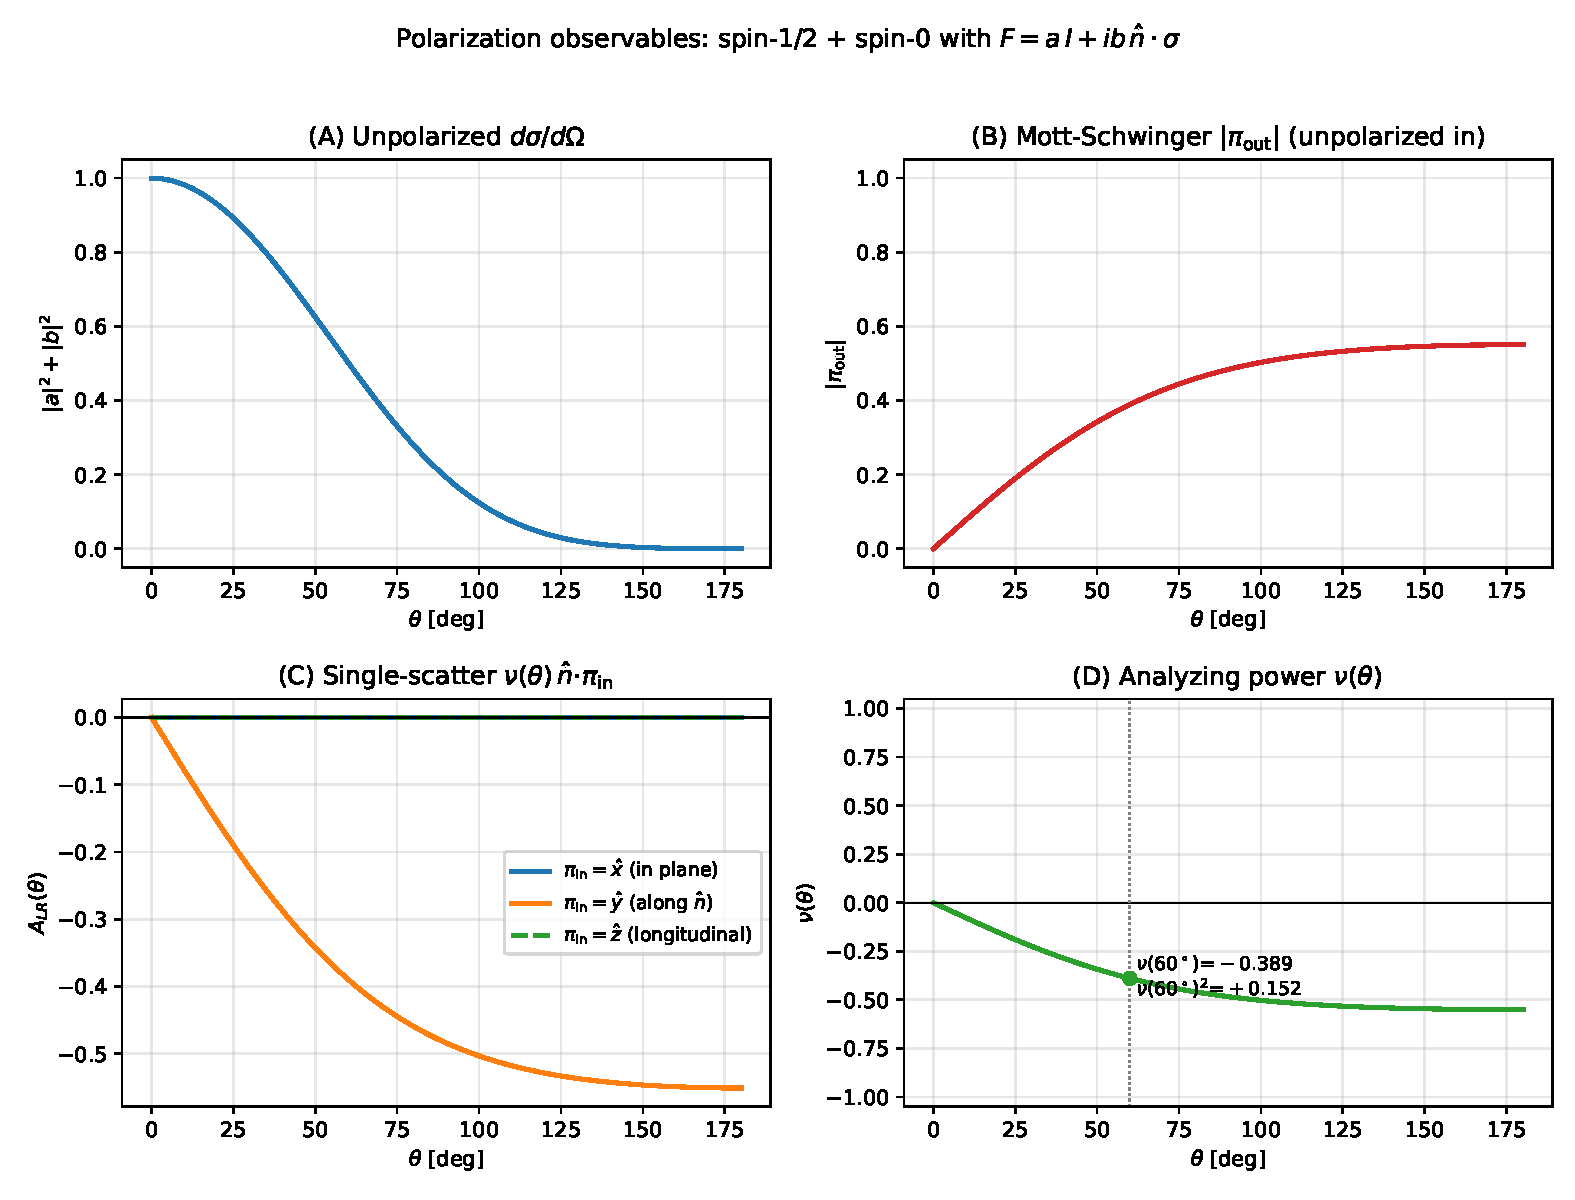
\includegraphics[width=0.95\linewidth]{ch04_polarization}
    \caption{自旋 $1/2$ + 自旋 $0$ 极化观测量 (toy 振幅 $a,b$, $\phi=0$). (A) 非极化截面 $|a|^2+|b|^2$ 在前向 ($\theta\!\to\!0$) 集中, 这是 $a$ 中 $\cos(\theta/2)$ 与 Gauss 包络的合成. (B) 非极化入射的出射极化模 $|\bm\pi^{\rm out}|=|\nu|\le 1$, 极大值出现在中等角度——前向 $b\!\to\!0$ 与后向 Gauss 阻尼都使 $\nu\!\to\!0$. (C) 单次散射 $A_{\rm LR}$: $\bm\pi^{\rm in}=\hat{\bm y}$ (沿 $\hat{\bm n}$) 给出非零信号 $=\nu(\theta)$; $\bm\pi^{\rm in}=\hat{\bm x},\hat{\bm z}$ 严格为零, 数值上验证了式 \eqref{eq:spin2p-ex1-general}. (D) analyzing power $\nu(\theta)$: 在 $60^\circ$ 处 $\nu\!\approx\!-0.389$, 对应对称双散射 ($\hat{\bm n}_2=+\hat{\bm n}_1$) 的 $A_{\rm LR}=\nu^2\!\approx\!+0.152$.}\label{fig:numexp-ch04}
\end{figure}

\subsection*{物理讨论}
\begin{itemize}\itemsep=2pt
  \item \textbf{$\hat{\bm n}$ 方向的特殊地位.} 图 (C) 三条曲线同时绘出, 但只有 $\bm\pi^{\rm in}=\hat{\bm y}$ 那一条非零. 这是 \eqref{eq:spin2p-ex1-general} 中 $A_{\rm LR}\propto\hat{\bm n}\!\cdot\!\bm\pi^{\rm in}$ 的直接体现: 散射平面内的极化 ($\hat{\bm x},\hat{\bm z}$) 不耦合到 single-scatter asymmetry, 平面外法向极化 ($\hat{\bm y}$) 才耦合. 这是 \emph{宇称}与 \emph{旋转不变性}的联合后果——$F$ 中能出现的唯一 $\bm\sigma$ 组合就是 $\hat{\bm n}\!\cdot\!\bm\sigma$ (轴向赝矢量).
  \item \textbf{Cross section vs.\ 极化的互补性.} 图 (A) 与 (D) 各自只看到一半信息: 非极化截面 $|a|^2+|b|^2$ 完全不含 $\arg(ab^*)$, 而 analyzing power $\nu\propto\Im(ab^*)$ 恰好提取相位差. 实验上若只测 $\rmd\sigma/\rmd\Omega$ 不可能拆出 $a,b$; 测了 $\nu$ (双散射或极化靶) 才能反演振幅相位.
  \item \textbf{相位 0.6 的角色.} 把代码中 $b(\theta)$ 的 $\rme^{\rmi\,0.6}$ 改成 $\rme^{\rmi\,0}$ 会让 $\nu\equiv 0$, (B)(C)(D) 整体塌缩到零线 (而 (A) 几乎不变). 这从数值上展示了 \emph{极化观测量是相位敏感探针}.
  \item \textbf{双散射放大.} $\nu(60^\circ)\!\approx\!-0.39$ 在单次散射截面里被 $|a|^2+|b|^2$ 平均掉, 不可观测; 但接成 $\theta_1=\theta_2=60^\circ$ 的双散射后 $A_{\rm LR}=\nu^2\!\approx\!0.15$ ($\sim 15\%$) 直接出现在左/右探测器的计数差异中——这就是 Mott (1929--32), Schwinger (1948) 测量 spin--orbit 振幅相位的实验原理.
  \item \textbf{扩展.} 把 $a,b$ 换成真实物理输入 (如 partial-wave 展开 $a=\sum_\ell[(\ell+1)f_\ell^++\ell f_\ell^-]P_\ell$, $b$ 为相应的 spin-flip 组合) 即可对真实弹性散射做同样的分析. 第\ref{ch:morespin}章会扩展到自旋 $1/2$ + 自旋 $1/2$, 此时 $F$ 含 $5$ 个独立 Wolfenstein 振幅, 极化观测量集合也相应丰富.
\end{itemize}
